\documentclass[12pt]{article}
\usepackage{amsmath,amssymb}
\textwidth=167mm \textheight=250mm \oddsidemargin -0.2 cm\evensidemargin -0.2cm \topmargin -2.5cm
\renewcommand\baselinestretch{1.2}
\renewcommand{\thesection}{}
\renewcommand{\thesubsection}{\arabic{section}.\arabic{subsection}.}
\renewcommand{\thesubsubsection}{\arabic{section}.\arabic{subsection}.\arabic{subsubsection}.}

\usepackage[cp1251]{inputenc}
\usepackage{graphicx,caption2}


\def\na{{\mbox{\boldmath$\nabla$}}}
\def\br{{\mbox{\boldmath$r$}}}
\def\bp{{\mbox{\boldmath$p$}}}
\def\bq{{\mbox{\boldmath$q$}}}
\begin{document}

\thispagestyle{empty}
\begin{center}
\Large{Bonn-Colonge Graduated School of Physics and Astronomy \\
Rheinische Friedrich-Wilhelms-Universitat Bonn}

\vspace*{6.1 cm}
\textbf{\LARGE{Stars and Stellar Evolution\\ Laboratory Work\\[2mm]}}
\textbf{\large{Vsevolod Nedora\\}}
\vspace*{11 cm} \Large{Bonn, 2016-2017}
\end{center}

\newpage

\section{Excercise 1}

In this exercise the $1M_\odot$ model of a star is being evolved. Given initial  metallicity $Z=0.02$. Initial structure is taken from \emph{ZAMS} stars bank. 
The program was terminated after $N=857$ iterations. The HDR of this model is presented in figure \ref{fig:HDR}.
\begin{figure}[ht]
\begin{center}
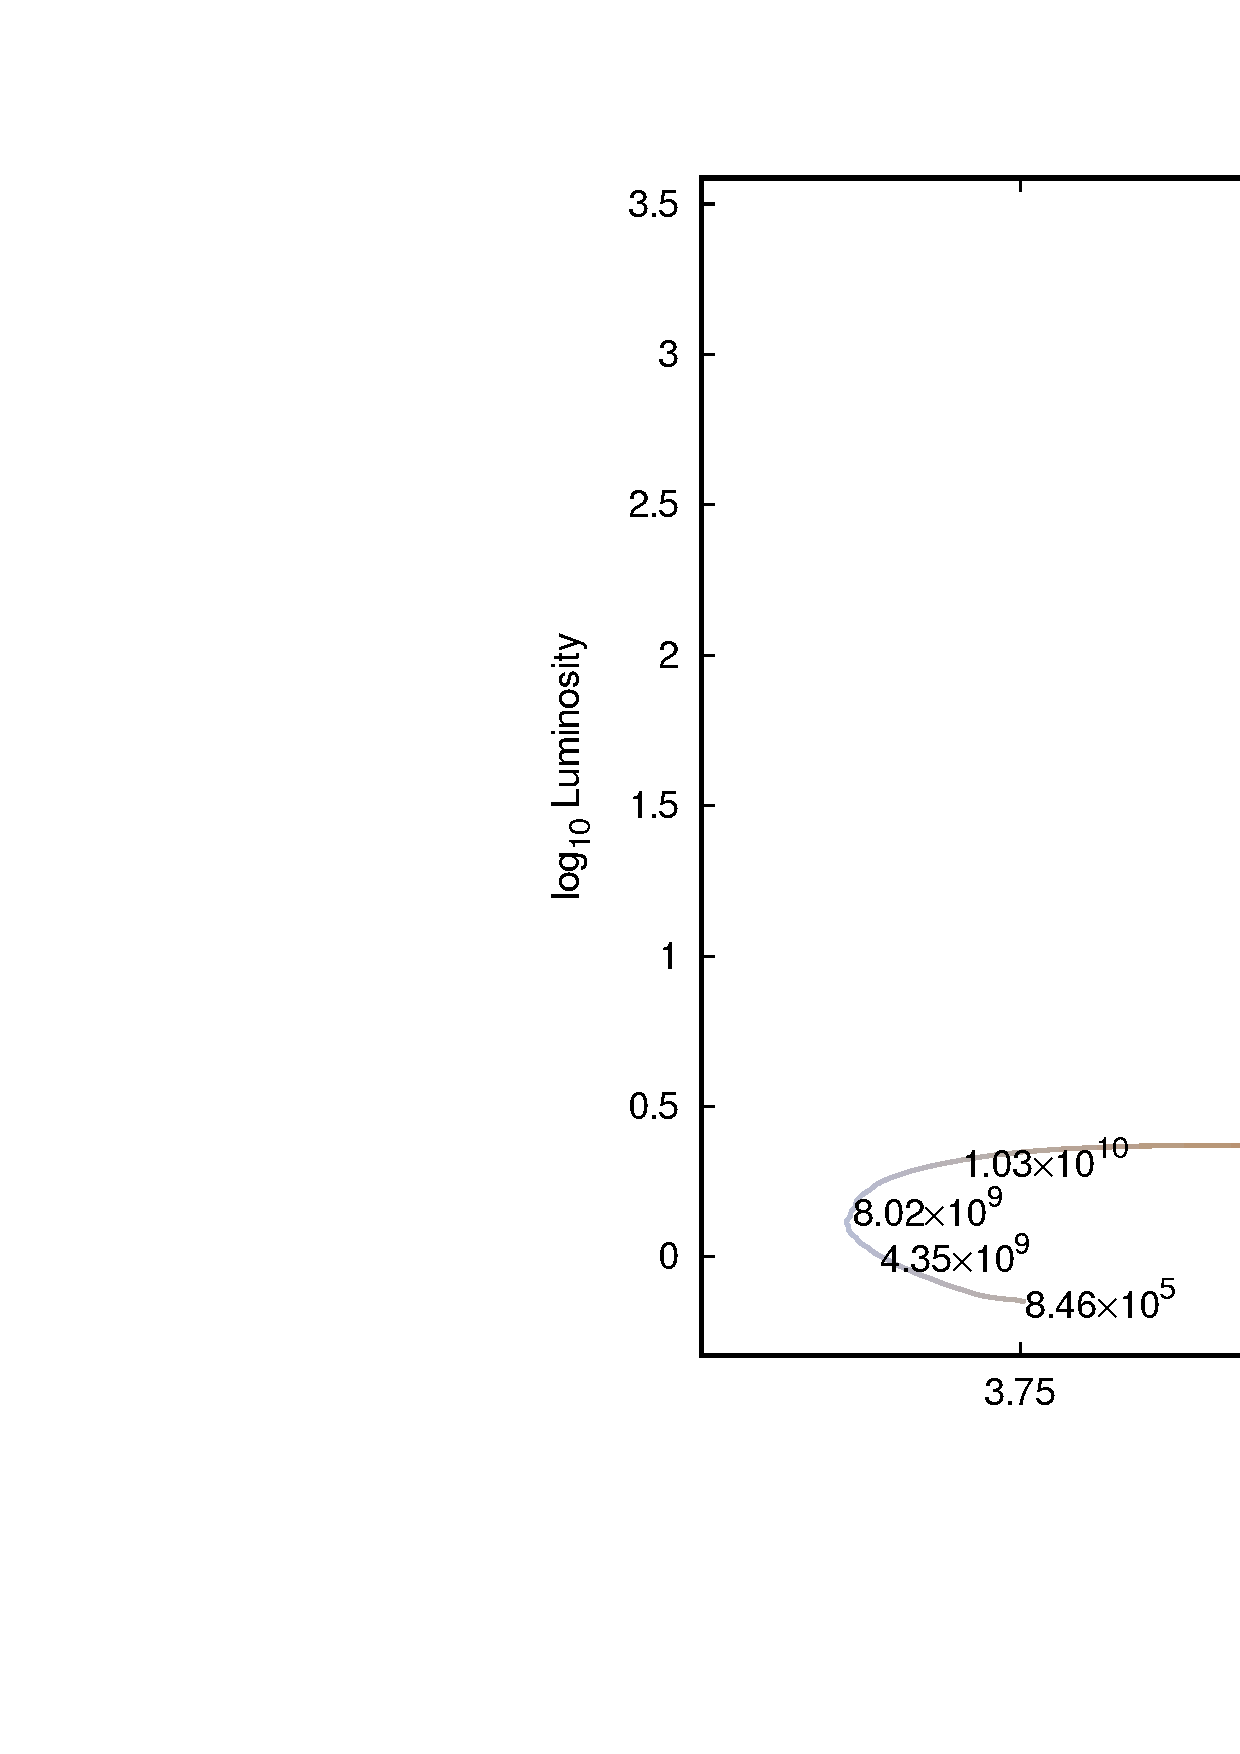
\includegraphics[width=1.0\textwidth]{hrd.png}
\end{center}
\vspace*{-10mm}
\caption{Hertzsprung-Russell-Diagram of a $1M_\odot$ star. Labels corresponds to a star age.}
\label{fig:HDR}\end{figure}
\subsection{}

\paragraph{a)}
The starting model has following characteristic values: effective temperature $T_{eff}=5623K$ and luminosity $L=0.7L_{\odot}$. These values were obtained from program log.
\begin{figure}[ht]
\begin{center}
\includegraphics[width=1.0\textwidth]{T_vs_L}
\end{center}
\vspace*{-10mm}
\caption{$T_{eff}$ vs $L$}
\label{fig:Teff_vs_L}
\end{figure}
\paragraph{b)}

From the \ref{fig:Teff_vs_L} it is visible that the maximum effective temperature this model reaches is $T_{eff}=5840K$, luminosity at this point is $L=1.3L_{\odot}$.

\subsection{}
To locate the point in the HRD corresponding to the Sun we must locate point, where $\log \frac{L}{L_{\odot}} = 0$. Zoomed in plot of this section of HRD is given in 

\begin{figure}[ht]
\begin{center}
\includegraphics[width=1.0\textwidth]{ex_1_2.png}
\end{center}
\vspace*{-10mm}
\caption{HRD near the Sun}
\label{fig:HRD_sun}
\end{figure}
\paragraph{a)}
Approximate age is $4.3 \, Gyr$.
\paragraph{b)}
Effective temperature at this point is $T_{eff}=5800K$.
\paragraph{c)}
Current measured age of the Sun is $4.57 \,\pm \,0.1 \,Gyr$ and effective temperature $T_{eff}=5778K$. Numbers obtained from simulation are pretty close to this values with very small deviations and provides good model for the Sun.

\subsection{}


\paragraph{a)}
From figure \ref{fig:ex_1.3_a1} it is shown that Model number 47 has the Sun's luminosity. Its age is $4.1 \, Gyr$ as seen from figure \ref{fig:ex_1.3_a2}.

\begin{figure}[ht]
\begin{center}
\includegraphics[width=1.0\textwidth]{ex_1_3_b.png}
\end{center}
\vspace*{-10mm}
\caption{}
\label{fig:ex_1.3_b}
\end{figure}

\paragraph{b)} 

Figure \ref{fig:ex_1.3_b} shows that at age zero central temperature is $T_c=1.34 \cdot 10^7 K$ .

\paragraph{c)}
As seen from exercise 2 age of the model is in good correspondance to the age of the actual Sun, so we can define 'most like' model as this one and calculate central temperature at that age, which is $4.3 Gyr$  and $T_c=1.56 \cdot 10^7 K$. 

\begin{figure}[!ht]
\begin{center}
\includegraphics[width=1.0\textwidth]{ex_1_3_d.png}
\end{center}
\vspace*{-10mm}
\caption{}
\label{fig:ex_1.3_d}
\end{figure}

\paragraph{d)}
From figure \ref{fig:ex_1.3_d} we see that central Helium supply exhausts after $t\approx 8.9 Gyr$. 

\paragraph{e)}

After H is depleted in star's core at around age $t\approx 8.9 Gyr$ central temperature first grows slowly  as seen from figure \ref{fig:ex_1.3_e} ,because it does not immediately react to disturbance of TE, and then rises rapidly. The latter happens ,because star can not counteract gravity pressure anymore and it starts to collapse ,which increases internal energy ,and therefore central temperature, of the core according to the virial theorem. This collapse continues until enough central temperature is achieved to ignite helium fusion at $T\approx 10^8 K$ and stabilize collapse.

\subsection{}
\begin{figure}[!ht]
\begin{center}
\includegraphics[width=1.0\textwidth]{ex_1_4.png}
\end{center}
\vspace*{-10mm}
\caption{}
\label{fig:ex_1.4}
\end{figure}
\paragraph{a)}
Star passes through current solar radius at $\log{(R/R_{\odot})}=0$ corresponding to the age $4.49 Gyr$.
\paragraph{b)}
Age obtained from radius is closer to the actual solar age than age obtained from solar luminosity. So this model does not perfectly describe the Sun, but it is still pretty good approximation.
\paragraph{c)}
Tuning initial conditions that can match zero age Sun might improve results. One of the effect is convective overshoot, which causes cool sinking material from convective zone to penetrate into the radiative zone, which affects heat transfer rate and the central temperature. Overshooting causes the core mass to appear larger than at end of the main sequence than it is expected.

\subsection{}
\begin{figure}[!ht]
\begin{center}
\includegraphics[width=1.0\textwidth]{ex_1_5.png}
\end{center}
\vspace*{-10mm}
\caption{}
\label{fig:ex_1.5}
\end{figure}

\paragraph{a)}
Abundances are $A_O=1\%$, $A_C=0.28\%$ and $A_N=0.2\%$. Their sum is $1.48\%$.
\paragraph{b)+c)}
Early on Carbon abundance drops, because it is turned into Nitrogen with reaction $^{12}C(p,\gamma)^{13}N$. This can be seen from figure \ref{fig:ex_1.5}, where abundance of N is increasing while abundance of C decreases. This reaction is part of the CNO-I cycle, main product of which is $\alpha-particle$.
\paragraph{d)+e)}
After $6Gyr$ Oxygen abundance starts to drop sharply, while Nitrogen abundance grows at the same time. This is caused by CNO-II cycle in which Oxygen is turned into Nitrogen. Main product of this cycle is still $\alpha-particle$. It does not happen earlier because Oxygen has higher Coulomb barrier than Nitrogen and Carbon. Its Gamow peak, which defines maximum of reaction rate, is located at higher temperatures and this reaction becomes relevant in later stages of star's evolution, when central temperature becomes high enough.
\paragraph{f)}
The sum $C+N+O$ at ages 0,5 and 10 Gyr are $1.48\%$, $1.51\%$ and $1.45\%$ respectively. In CNO cycle C,N and O acts as a catalyst for reaction $4p\longrightarrow\alpha$ and their total number is conserved. Because of convective mixing, which brings heavy nuclei from surface to core and and vice versa, total abundance might not stay quite constant.
 
\newpage

\section{figures}

\begin{figure}[!ht]
\begin{center}
\includegraphics[width=1.0\textwidth]{ex_1_3_a1.png}
\end{center}
\vspace*{-10mm}
\caption{}
\label{fig:ex_1.3_a1}
\end{figure}

\begin{figure}[!ht]
\begin{center}
\includegraphics[width=1.0\textwidth]{ex_1_3_a2.png}
\end{center}
\vspace*{-10mm}
\caption{}
\label{fig:ex_1.3_a2}
\end{figure}

\begin{figure}[!ht]
\begin{center}
\includegraphics[width=1.0\textwidth]{ex_1_3_e.png}
\end{center}
\vspace*{-10mm}
\caption{}
\label{fig:ex_1.3_e}
\end{figure}

\end{document}